\documentclass{standalone}
\usepackage{amssymb,amsmath,latexsym, braket}
\usepackage{tikz, pgfplots, graphicx}
\begin{document}
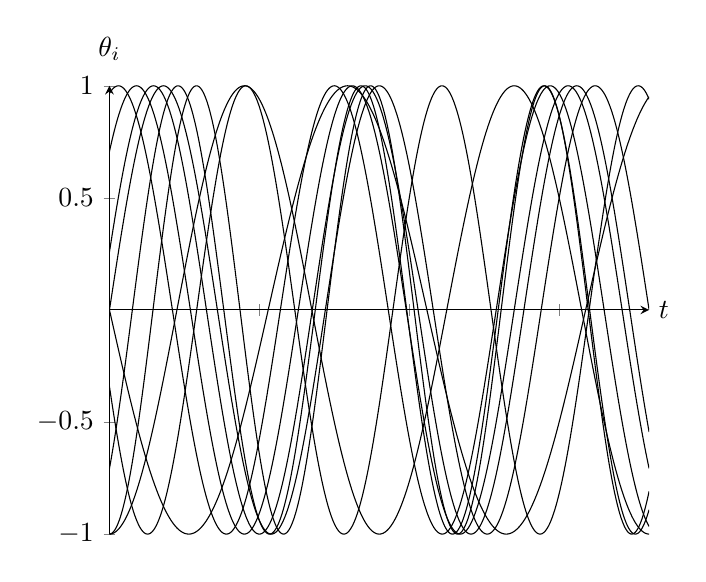
\begin{tikzpicture}
    \begin{axis}[domain=0:180,legend pos=south east,
    axis lines*=middle,
    xlabel=$t$,
    ylabel=$\theta_i$,
    xtick={},
    xticklabels={},
    axis lines = middle,
every axis x label/.style={at={(current axis.right of origin)},anchor=west},
every axis y label/.style={at={(current axis.north west)},above=2mm},
     ]
    \addplot[samples=500, mark=none] {sin(5*x)};
    \addplot[samples=500, mark=none] {sin(4*x + 270)};
    \addplot[samples=500, mark=none] {sin(5.1*x + 15)};
    \addplot[samples=500, mark=none] {sin(5.5*x + 200)};
    \addplot[samples=500, mark=none] {sin(6.2*x - 90)};
    \addplot[samples=500, mark=none] {sin(5.9*x - 45)};
    \addplot[samples=500, mark=none] {sin(5*x + 75)};
    \addplot[samples=500, mark=none] {sin(3.4*x + 180)};
    \addplot[samples=500, mark=none] {sin(5*x + 45)};
    \end{axis}
\end{tikzpicture}
\end{document}